\documentclass{beamer}
%\usepackage[all,arc,curve,frame,color]{xy}
%\usepackage{tkz-graph}
\usepackage{mathtools}
\usepackage{ragged2e,etoolbox}


\newenvironment{nstabbing}
  {\setlength{\topsep}{0pt}%
   \setlength{\partopsep}{0pt}%
   \tabbing}
  {\endtabbing}

\def\jump{ \quad \\ \vspace{0.7cm} \pause}
\newcommand{\nc}{\newcommand}
\nc{\pid}{\mathfrak{p} }
\nc{\dpid}{\delta_{\mathfrak{p}}}

\def\AA{{\mathbb A}}
\def\CC{{\mathbb C}}
\def\EE{{\mathcal E}}
\def\FF{{\mathcal F}}
\def\GG{{\mathcal G}}
\def\HH{{\mathcal H}}
\def\MM{{\mathcal M}}
\def\NN{{\mathbb N}}
\def\PP{{\mathbb P}}
\def\QQ{{\mathbb Q}}
\def\RR{{\mathbb R}}
\def\ZZ{{\mathbb Z}}
\def\aa{{\mathbf a}}
\def\bb{{\mathbf b}}
\def\del{\partial}
\def\kk{\Bbbk}
\def\mm{{\mathfrak m}}
\def\nn{{\mathfrak n}}
\def\pp{{\mathfrak p}}
\def\qq{{\mathfrak q}}
\def\rr{{\mathbf r}}
\def\uu{{\mathbf u}}
\def\vv{{\mathbf v}}
\def\ww{{\mathbf w}}
\def\xx{{\mathbf x}}
\def\yy{{\mathbf y}}
\def\zz{{\mathbf z}}
\newcommand{\PGL}{\textrm{PGL}}
\newcommand{\res}{\textrm{Res}}


\DeclareMathOperator{\Tail}{Tail}
\DeclareMathOperator{\Per}{Per}
\DeclareMathOperator{\PrePer}{PrePer}
\DeclareMathOperator{\HTail}{HTail}
\DeclareMathOperator{\HPer}{HPer}
\DeclareMathOperator{\HPrePer}{HPrePer}

\makeatletter
\def\th@mystyle{%
    \normalfont % body font
    \setbeamercolor{block title example}{bg=orange,fg=white}
    \setbeamercolor{block body example}{bg=orange!20,fg=black}
    \def\inserttheoremblockenv{exampleblock}
  }
\makeatother

\makeatletter
\def\th@thmstyle{%
    \normalfont % body font
    \setbeamercolor{block title example}{bg=blue,fg=white}
    \setbeamercolor{block body example}{bg=blue!20,fg=black}
    \def\inserttheoremblockenv{exampleblock}
  }
\makeatother

\definecolor{darkgreen}{RGB}{77,153,0}
\makeatletter
\def\th@qstnstyle{%
    \normalfont % body font
    \setbeamercolor{block title example}{bg=darkgreen,fg=white}
    \setbeamercolor{block body example}{bg=green!20,fg=black}
    \def\inserttheoremblockenv{exampleblock}
  }
\makeatother

\theoremstyle{thmstyle}
\newtheorem*{mydef}{Definition}

\theoremstyle{thmstyle}
\newtheorem*{mythm}{Theorem}

\theoremstyle{mystyle}
\newtheorem*{remark}{Remark}
\newtheorem*{conjecture}{Conjecture}
\newtheorem*{mycor}{Corollary}
\newtheorem*{mylemma}{Lemma}

\theoremstyle{qstnstyle}
\newtheorem*{question}{Question}

\usepackage{remreset}% tiny package containing just the \@removefromreset command
\makeatletter
\@removefromreset{subsection}{section}
\makeatother
\setcounter{subsection}{1}

\newcommand\Wider[2][3em]{%
\makebox[\linewidth][c]{%
  \begin{minipage}{\dimexpr\textwidth+#1\relax}
  \raggedright#2
  \end{minipage}%
  }%
}

\mode<presentation>{\usetheme{CambridgeUS}\usecolortheme{dolphin}} 
%\setbeamertemplate{navigation symbols}{}
\setbeamertemplate{blocks}[rounded][shadow=false]


\title[Preperiodic Hypersurfaces]{$K$-rational preperiodic hypersurfaces on $\PP^n$}
%\subtitle[Dissertation Defense]{Dissertation Defense}
\author[S. Troncoso]{Sebastian Troncoso}
\institute[MSU $\rightarrow$ BSC]{Michigan State University\\ $\downarrow$ \\ Birmingham-Southern College}
%\titlegraphic{\includegraphics[height=1.5cm]{../images/normale_pisa.png}}
\date[July 4, 2017.]{ July 4, 2017. \\ \vspace{1cm} }


%\AtBeginSection[]{} % for optional outline or other recurrent slide
\AtBeginSection{\frame{\sectionpage}}
\begin{document}

\begin{frame}
\titlepage
\end{frame}

\begin{frame}
\frametitle{Notation}
Let $K$ be a number field  and $\mathcal{O}_K$ its ring of algebraic integers,
\\\quad\\
\pause
$\phi:\mathbb{P}^n\to\mathbb{P}^n$ be an endomorphism defined over $K$ \\ $\phi^m$ the $m$th iterate
of $\phi$.
\\\quad\\
\pause
The \textbf{orbit} of a point $P\in\PP^n$ is the set 
$$ O_{\phi}(P) = \{P, \phi(P),\phi^2(P),\phi^3(P),\ldots \}.$$

%\pause The \textbf{orbit length} of $P$ is the cardinality of the orbit of $P$ (as a set).
\end{frame}


\begin{frame}
\frametitle{Notation}

\textbf{Periodic point}: $\phi^m(P)=P$ for some $m\geq{1}$.
\\\quad\quad \pause Minimal $m$ is called the \textbf{period} of $P$.

\pause
\vspace{2mm}
The set of $K$-rational periodic points for $\phi$ is denoted by $\Per(\phi,K)$.
\\\quad\\
\pause
\textbf{Preperiodic point}: $\exists m\geq{0}$ such that $\phi^m(P)$
is periodic \\\quad\quad \pause \emph{i.e.}  $P$ has finite orbit.

\pause
\vspace{2mm}
The set of $K$-rational preperiodic points for $\phi$ is denoted by $\PrePer(\phi,K)$.
\\\quad\\
\pause
\textbf{Tail point}: A point that is preperiodic but not periodic.

\pause
\vspace{2mm}
The set of $K$-rational tail points for $\phi$ is denoted by $\Tail(\phi,K)$.
\end{frame}

\begin{frame}
\frametitle{Examples:}
We can view $\PP^1(K)$ as $K\cup \{\infty \}$ and endomorphism of $\PP^1$ as rational functions.

\begin{center}
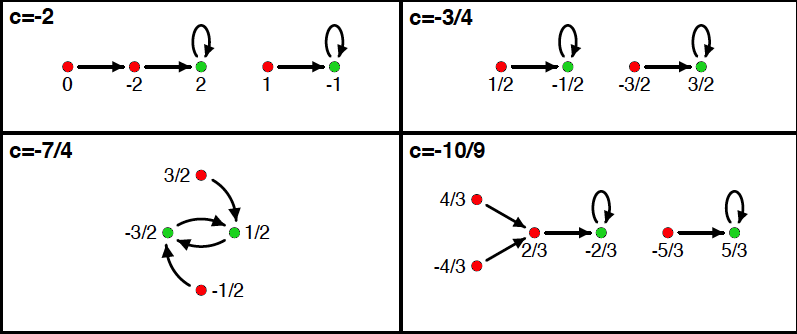
\includegraphics[width=1.0\linewidth]{placeholder4}
\end{center}

$\QQ$-rational tail points (red) and $\QQ$-rational periodic points (green) of  $\phi_c(z)=z^2+c$.
\end{frame}


\begin{frame}
\frametitle{Question:}
\begin{itemize}
\item Are the sets $\Tail(\phi,K)$, $\Per(\phi,K)$ and $\PrePer(\phi,K)$ finite? 

\pause \textbf{Yes}. 
\vspace{6mm}\pause

\begin{mythm}[Northcott 1950]
Let $\phi : \PP^n \to \PP^n$ be an endomorphism of degree $\geq{2}$
defined over a number field $K$. Then $\phi$ has
only finitely many preperiodic points in $\PP^n(K)$.
\end{mythm}

\vspace{6mm} \pause
We can deduce from the original proof of Northcott's theorem  a bound for $|\PrePer(\phi,K)|$ depending on
\begin{itemize}
\item $n$
\item $[K:\QQ]$
\item the degree of $\phi$
\item height of the coefficients of $\phi$
\end{itemize}
\end{itemize}
\end{frame}

\begin{frame}
\frametitle{Goals:}
Give explicit bounds for $|\Tail(\phi,K)|$, $|\Per(\phi,K)|$ and $|\PrePer(\phi,K)|$ in terms of:\pause
\begin{itemize}
\item  $D=[K: \QQ]$\pause 

\item The dimension $n$ of the projective space \pause 

\item The degree $d$ of $\phi$.
\end{itemize}

\pause

\begin{conjecture}[Uniform Boundedness Conjecture - Morton--Silverman
  1994]
There exists a bound $B = B(D,n,d)$ such that if $K/\mathbb{Q}$ is a number field of degree $D$, and $\phi:\mathbb{P}^n\rightarrow\mathbb{P}^n$ is an endomorphism of degree $d\geq{2}$ defined over $K$, then 
$$|\text{PrePer}(\phi,K)| \leq B.$$
\end{conjecture}
\end{frame}

\begin{frame}
\frametitle{Goals:}

In order to get explicit bounds for the cardinality of the set $\PrePer(\phi,K)$ we need an extra parameter. 

Instead of the height of $\phi$ we can use a weaker and more natural parameter to get bound on $|\PrePer(\phi,K)|$.\pause 

This parameter is the number of places of bad reduction of $\phi$.


\jump

Give explicit bounds for $|\Tail(\phi,K)|$, $|\Per(\phi,K)|$ and $|\PrePer(\phi,K)|$ in terms of:
\begin{itemize}
\item  $D=[K: \QQ]$ 

\item The dimension $n$ of the projective space  

\item The degree $d$ of $\phi$.

\item The number of places of bad reduction of $\phi$.
\end{itemize}


\end{frame}

%\begin{frame}
%\frametitle{Normalized Form and Good Reduction}
%Let $\phi$ be an endomorphism of $\PP^n$ defined over $K$, $\mathfrak{p}$ be a non zero prime ideal of $\mathcal{O}_K$
%, $\mathcal{O}_{\mathfrak{p}}$ the local ring at $\pid$ and $k=\mathcal{O}_{\mathfrak{p}}/\pid$ the residue field of $\mathcal{O}_{\mathfrak{p}}$. Let $F_0,\ldots,F_n \in K[X_0,\ldots,X_n]$ be homogeneous polynomials of the same degree with no common zero on $\PP^n$ \jump
%
%
%\begin{itemize}
%\item We say that $\phi=[F_0,\ldots, F_n]$ is in  \textbf{normalized form} with respect to $\pid$ if  all the coefficients of $F_0,\ldots,F_n$ are in $\mathcal{O}_\pid$ and at least one is a $\pid$-unit. \jump
%\item For an any representation $\phi=[F_0,\ldots, F_n]$ we can find a $c\in K^{*}$ such that $[cF_0,\ldots, cF_n]$ is in normalized form with respect to $\pid$.
%\end{itemize}
%\end{frame}
%
%\begin{frame}
%\frametitle{Normalized Form and Good Reduction}
%
%\begin{itemize}
%\item Write $\phi=[F_0,\ldots, F_n]$ in normalized form with respect to $\pid$. Consider the reduction of $\phi$ modulo $\pid$ given by
%$$\tilde{\phi}=[\tilde{F_0},\ldots,\tilde{ F_n}] $$
%In other words, $\tilde{\phi}$ is obtained by reducing the coefficients of $F_0,\ldots,F_n$ modulo $\pid$.
%\jump
%Then $\phi$ has \textbf{good reduction} at $\pid$ if the system of equations $\tilde{F_0}=\ldots=\tilde{F_n}=0$ have no common zero in $\mathbb{P}^n(\bar{k})$.
%
%\jump
%\item $\phi$ has \textbf{bad reduction} at $\pid$ if it does not have good reduction at $\pid$.
%\end{itemize}
%\end{frame}

\begin{frame}
\frametitle{Good Reduction}
Let $S$ be a finite set of places $K$, including all archimedean ones.
\jump
\begin{itemize}
\item We say that $\phi$  has \textbf{good reduction outside} $S$ if $\phi$ has good reduction for every $\pid \notin S$.

\jump
\end{itemize}

If we allow the number of primes of bad reduction as a parameter, much more is known for the cardinality of the set of $K$-rational preperiodic points in the case of $\PP^1$. 
\end{frame}






%\begin{frame}
%\frametitle{Bound on maximal period}
%\begin{mythm}[W.\ Narkiewicz 1988]
%Let $\phi \in K[z]$ be a polynomial of degree $\geq{2}$
%defined over a number field $K$ of degree $D=[K:\QQ]$. 
%Suppose $\phi$ has good reduction outside a finite set of places $S$, including all archimedean ones. Let $s=|S|$.
%\\\quad\\
%If $P$ is a $K$-rational periodic point of period $n$, then
%$$ n \leq (6\cdot 7^{D+2s})^\alpha,$$ where $\alpha=O(s\log{s}).$
%\end{mythm}
%\end{frame}




%\begin{frame}
%\frametitle{Bound on maximal orbit length of a preperiodic point}
%\begin{mythm}[J.K.\ Canci 2006]
%Let $\phi : \PP^1\to\PP^1$ be a rational map of degree at least two
%defined over a number field $K$. 
%Suppose $\phi$ has good reduction outside a finite set of places $S$, including all archimedean ones. Let $s=|S|$.
%\\\quad\\
%If $P\in\text{PrePer}(\phi,K)$ is of orbit length $n$, then
%$$n\leq\left[{e^{10}}^{12}(s+1)^8(log(5(s+1)))^8\right]^s.$$
%\end{mythm}
%\end{frame}

%\begin{frame}
%\frametitle{Bound on maximal orbit length of a preperiodic point }
%\begin{mythm}[J.K.\ Canci, L.\ Paladino 2015]
%Let $\phi : \PP^1\to\PP^1$ be a rational map of degree $\geq{2}$
%defined over a number field $K$ and $[K: \mathbb{Q}]=D$. 
%Suppose $\phi$ has good reduction outside a finite set of places $S$, including all archimedean ones. Let $s=|S|$.
%If $P\in\text{PrePer}(\phi,K)$ is of orbit length $n$, then
%$$n\leq \max\left\{(2^{16s-8}+3)\left[12s\log(5s)\right]^{D}, \left[12(s+2)\log(5s+5)\right]^{4D}\right\}
%.$$
%\end{mythm}
%\jump
%From here we can deduce a bound for $|\PrePer(\phi,K)| $ that is roughly of the order $\displaystyle d^{2^{16s}\left( s\log(s) \right)^{D}}$.
%
%\end{frame}




%\begin{frame}
%\frametitle{From bound of maximal period to bound of $\#\text{Per}(\phi,K)$}
%
%\begin{remark}
%
%Given a bound on the maximal period of a $K$-rational periodic point, we can get a (naive) bound on the number of periodic points, as any periodic point of period $\leq{N}$ satisfies some equation $f^n(P)=P$ for $1\leq{n}\leq{N}$.
%
%\quad \\
%
%We can get in this way a bound that is on the order of $O(d^N)$, where $N$ is the maximal possible period.
%\end{remark}
%\end{frame}

%\begin{frame}
%\frametitle{Best \textbf{full} bound (so far) for polynomials}
%\begin{mythm}[R.L.\ Benedetto 2007]
%Let $\phi \in K[z]$ be a polynomial of degree $d\geq{2}$
%defined over a number field $K$ of degree $D=[K:\QQ]$. 
%Suppose $\phi$ has good reduction outside a finite set of places $S$, including all archimedean ones. Let $s=|S|$.
%The number of preperiodic points of $\phi$ in $\PP^1(K)$ is at most $O(s\log s)$ and $O(d^2/\log{d})$. 
%\end{mythm}
%
%\pause
%
%\begin{itemize}
%\item Proved by using nonarchimedean places $\nu$ of bad reduction and bounding the filled Julia set in the completion $K_\nu$.  \pause
%\item X.\ Faber (2015) used ``Benedetto's trick'' to find exact number of preperiodic points in certain infinite sequences of quadratic polynomials.
%\end{itemize}
%\end{frame}





\begin{frame}
\frametitle{Bounds independent of the degree}
\begin{mythm}[S.\ Troncoso 2016]
Let $K$ be a number field and $S$ a finite set of places of $K$ containing all the archimedean ones. Let $\phi $ be an endomorphism of $\PP^1$, defined over $K$, and $d \geq 2$ the degree of $\phi$. Assume $\phi$ has  good reduction outside $S$.
\begin{enumerate}

\item [(a)] 
If there are at least three $K$-rational tail points of $\phi$ then
$$|\Per(\phi,K)| \leq 2^{16|S|}+3. $$

\item [(b)]
If there are at least four $K$-rational periodic points of $\phi$ then
$$|\Tail(\phi,K)| \leq 4(2^{16|S|}).$$
\end{enumerate}
\end{mythm}
\pause
Notice that under these hypotheses the bounds are independent of the degree of $\phi$. Those hypotheses are sharp, \emph{i.e.} if there are two (three) $K$-rational tail (periodic) points then $|\Per(\phi,K)|$ ($|\Tail(\phi,K)|$) must depend on $d$. 
\end{frame}

\begin{frame}
\frametitle{Distance between periodic and tail points}
\begin{mythm}[S.\ Troncoso 2016]
Let $\phi$ be an endomorphism of $\PP^1$, defined over $K$. Suppose $\phi$ has good reduction outside $S$. Let $R\in\PP^1(K)$ be a tail point and let $n$ be the period of the periodic part of the orbit of $R$. Let $P\in\PP^1(K)$ be any periodic point that is not $\phi^{mn}(R)$ for some $m$. Then $\delta_\pp(P,R)=0$ for every $\pp \notin S$.
\end{mythm}

For simplicity suppose $\mathcal{O}_S$ is a PID and write $P=[x:y]$ and $Q=[w:t]$ in coprime $S$-integer coordinates.

\pause Using the theorem we get that there is a $S$-unit element $u$ such that
$$xt-yw=u $$
\end{frame}

\begin{frame}
\begin{mythm}[S.\ Troncoso 2016]
Let $K$ be a number field and $S$ a finite set of places of $K$ containing all the archimedean ones. Let $\phi $ be an endomorphism of $\PP^1$, defined over $K$, and $d \geq 2$ the degree of $\phi$. Assume $\phi$ has  good reduction outside $S$. Then
\begin{enumerate}
\item [(a)] $|\Per(\phi,K)| \leq  2^{16|S|d^3}+3.$

\item [(b)] $|\Tail(\phi,K)| \leq  4(2^{16|S|d^3}) .$

\item [(c)] $|\PrePer(\phi,K)| \leq 5(2^{16|S|d^3})+3.$

\end{enumerate}
\end{mythm}

Notice that the bounds obtained  in the theorem are a significant improvement from the previous bound given by Canci and Paladino which was of the order $\displaystyle d^{2^{16s}\left( s\log(s) \right)^{D}}$ for the set $|\PrePer(\phi,K)|$.

\end{frame}

%\begin{frame}
%\frametitle{logarithmic $p$-adic chordal distance}
%
%Let $K$ be a number field, and $\nu_{\pid}$ a valuation associated to a prime $\pid$ of $K$. 
%\quad \\ 
%
%Let $P=[X_1:Y_1], Q=[X_2:Y_2] \in \PP^1(K)$. Then
%
%\quad \\ \pause
%\textbf{logarithmic $p$-adic chordal distance}:
%
%$$\delta_{\mathfrak{p}}\,(P,Q)=v_{\mathfrak{p}}\,(X_1Y_2-X_2Y_1)-\min\{v_{\mathfrak{p}}(X_1),v_{\mathfrak{p}}(Y_1)\}-\min\{v_{\mathfrak{p}}(X_2),v_{\mathfrak{p}}(Y_2)\}$$
%\end{frame}

%\begin{frame}
%\frametitle{$S$-integral points}
%
%\begin{itemize}
%\item Let $P,Q \in \PP^1(K)$. Then $P\equiv{Q}\pmod{\pid}$ iff $\delta_\pid(P,Q)\geq{1}$. \jump
%\item Let $S$ be a finite set of places of $K$ containing all the archimedean ones. \jump
%\item $P$ is \textbf{$S$-integral} with respect to $Q$ iff $\delta_\pid(P,Q)=0$ for all $\pid\not\in{S}$. \jump
%% \item A finite point $P$ is an $S$-integer iff it is $S$-integral with respect to $\infty$.
%\end{itemize}
%\end{frame}


\begin{frame}
\frametitle{Another technique}

Using another technique we can get a better result in terms of $d$. \pause

\begin{mythm}[S.\ Troncoso 2016]
Let $K$ be a number field and $S$ a finite set of places of $K$ containing all the archimedean ones. Let $\phi $ be an endomorphism of $\PP^1$, defined over $K$, and $d \geq 2$ the degree of $\phi$. Assume $\phi$ has  good reduction outside $S$. Then

\begin{enumerate}

\item [(a)] $|\Tail(\phi,K) | \leq d\max\left\{  (5 \cdot 10^6 (d^3+1))^{|S|+4} ,4(2^{64(|S|+3)}) \right \}.$\jump

\item [(b)] In addition, if $\phi$ has at least one $K$-rational tail point then then
$$|\Per(\phi,K)| \leq   \max \left\{  (5 \cdot 10^6 (d-1))^{|S|+3} ,4(2^{128(|S|+2)}) \right\}+1.$$
\end{enumerate}
\end{mythm}
\end{frame}


%
%
%\begin{frame}
%\frametitle{Another technique: Thue-Mahler equations}
%Let $F(X,Y)$ be a binary  form of degree $r \geq 3$ with coefficients in $\mathcal{O}_S$  which is irreducible over $K$.\jump  An $\mathcal{O}_S^{*}$-coset of solutions of
%\begin{equation} \label{T-M}
% F(x,y) \in \mathcal{O}_S^{*}  \quad\quad \mbox{ in } \quad (x,y) \in \mathcal{O}_S^{2}
%\end{equation}
%is a set $\{\epsilon(x,y): \epsilon \in \mathcal{O}_S^{*} \}$, where $(x,y)$ is a fixed solution of (\ref{T-M}).
%\jump
%
%Evertse proved in 1997 that: the set of solutions of (\ref{T-M}) is the union of at most
%$$ (5\cdot 10^6r)^s$$
%$\mathcal{O}_S^{*}$-cosets of solutions.
%
%
%\end{frame}

\begin{frame}
\frametitle{Current project: Arithmetic dynamics in $\PP^n$.}


We are generalizing our results and techniques in $\PP^1$ into results and techniques in $\PP^n$.

\end{frame}

\begin{frame}
\frametitle{Notation of preperiodic hypersurfaces}
\pause
Let $\phi:\mathbb{P}^n\to\mathbb{P}^n$ be an endomorphism defined over $K$ and $H$ an irreducible hypersurface defined over $K$ of degree $e$.
\\\quad\\
\pause
The \textbf{orbit} of $H$ is the set 
$$ O_{\phi}(H) = \{H, \phi(H),\phi^2(H),\phi^3(H),\ldots \}.$$

%\pause The \textbf{orbit length} of $H$ is the cardinality of the orbit of $H$ (as a set).
\end{frame}


\begin{frame}
\frametitle{Notation of preperiodic hypersurfaces}

\textbf{Periodic hypersurface}: $\phi^m(H)=H$ for some $m\geq{1}$.
\\\quad\quad  Minimal $m$ is called the \textbf{period} of $H$.


\vspace{2mm}
The set of $K$-rational periodic hypersurface (of degree $e$) is denoted by $\HPer(\phi,K)$ ($\HPer(\phi,K,e)$).
\\\quad\\

\textbf{Preperiodic hypersurface}: $\exists m\geq{0}$ such that $\phi^m(H)$
is periodic \\\quad\quad  \emph{i.e.}  $H$ has finite orbit.


\vspace{2mm}
The set of $K$-rational preperiodic hypersurface (of degree $e$) is denoted by $\HPrePer(\phi,K)$ ($\HPrePer(\phi,K,e)$).
\\\quad\\

\textbf{Tail hypersurface}: A hypersurface that is preperiodic but not periodic.


\vspace{2mm}
The set of $K$-rational tail hypersurface (of degree $e$) is denoted by $\HTail(\phi,K)$ ($\HTail(\phi,K,e)$).
\end{frame}



\begin{frame}
\frametitle{Questions:}
\begin{itemize}
\item Are the sets $\HTail(\phi,K)$, $\HPer(\phi,K)$ and $\HPrePer(\phi,K)$ finite? 
\jump

\textbf{No}, an example by J. Bell, D. Ghioca, and T. Tucker have shown that in general these sets are not finite. 

\jump

\item Are the sets  $\HTail(\phi,K,e)$, $\HPer(\phi,K,e)$ and $\HPrePer(\phi,K,e)$ finite?

\pause \textbf{Yes}.


\end{itemize}

\end{frame}

\begin{frame}


\begin{mythm}[B. Hutz 2016]
Let $\phi : \PP^n \to \PP^n$ be an endomorphism of degree $\geq{2}$ defined over a number field $K$. Then there are only finitely many preperiodic $K$-rational subvarieties of degree at most $e$.
\end{mythm}

\jump 
His result is based on theory of canonical heights for subvarieties of $\PP^N$. From his proof we can give a bound for the cardinality of the set $\HPrePer(\phi,K,e)$ depending on
\begin{itemize}
\item $n$
\item $[K:\QQ]$
\item the degree of $\phi$
\item $e$
\item height of the coefficients of $\phi$
\end{itemize}
\end{frame}

\begin{frame}
\frametitle{Goals}
Just like the one dimensional case. 

We would like to give explicit bounds for the cardinality of the sets $\HTail(\phi,K,e)$, $\HPer(\phi,K,e)$ and $\HPrePer(\phi,K,e)$ in terms of:\pause
\begin{itemize}
\item  $D=[K: \QQ]$. 

\item The dimension $n$ of the projective space.  

\item The degree $d$ of $\phi$.

\item The degree $e$ of the hypersurfaces. \pause

\item  The number of places of bad reduction of $\phi$.
\end{itemize}


\end{frame}

\begin{frame}
\begin{itemize}
\item For now, we have just proven the following result for $\PP^2$.
\end{itemize}
\pause
If $T \in \HTail(\phi,K, e)$ then $n_T$ is the period of the periodic part of $T$. Consider $N$ the number of monomials of degree $e$ in three variables. \pause

\begin{mythm}[S.\ Troncoso 2017]
Let $\phi$ be an endomorphism of $\PP^2$, defined over $K$ and suppose $\phi$ has good reduction outside $S$. Let $\{P_i\}_{i=1}^{2N+1} $ be a set of $K$-rational periodic points of $\PP^2$. Assume that no $N+1$ of them lie in a curve of degree $e$. Consider $\mathcal{B} =\{ H^{\prime} \in \HPer(\phi,K) \colon \forall  1 \leq i \leq 2N+1 \quad P_i \notin  supp\ H^{\prime}     \} $ and $\mathcal{A}=\{ T \in \HTail(\phi,K, e) \colon \mbox{there is } l\geq 0 \quad \phi^{ln_T}(T) \in \mathcal{B}   \}$.  Then
 $$ |\mathcal{A} | \leq \left(2^{33} \cdot (2N+1)^2\right)^{\left(N+1\right)^3(s+2N+1)}  $$
\end{mythm}


\end{frame}

\begin{frame}
\begin{itemize}

\item  There is strong result from dynamical system that states that the set of periodic points is Zariski dense.

\jump 

\item On $\PP^2$. We can give an alternative proof than the one given by B. Hutz for the finiteness of the set $\HPrePer(\phi,K,e)$, 

\textbf{\emph{the idea}} is to use the previous theorem and the Zariski density of periodic points.
\end{itemize}
\end{frame}


\begin{frame}
\frametitle{Tools}
The theorem is based on the following three tools:\jump
\begin{itemize}
\item Logarithmic $v$-adic distance between a point and a hypersurface.


\jump

\item Study the distance between tail hypersurfaces and periodic points.

\jump

\item Finiteness of integral points of $\PP^n$ - $\{2n+1 \mbox{ hyperplanes in general position}\}$ due to Ru and Wong.



\jump

\item Bounds for the number of solutions to decomposable form equations (Evertse).
\end{itemize}
\end{frame}





\begin{frame}
\frametitle{logarithmic $v$-adic distance}
Let $H$ be a hypersurface of $\PP^n$ defined over $K$ of degree $e$.

\pause Further, suppose $H$ is defined by 

$$f=\displaystyle\sum_{|\textbf{i}|= d} a_{\textbf{i}}\textbf{X}^{\textbf{i}} \in K[\textbf{X}] $$ an homogeneous polynomial  of degree $e$. 

\pause Let $v$ be a nonarchimedean place of $K$ \pause and $P =[x_0:\cdots : x_n]$ a point in $\PP^n(K)$ \pause such that $P\notin supp(H) $. 
\jump
\textbf{logarithmic $v$-adic distance} between $P$ and $H$ with respect to $v$ is given by

$$\delta_{v}(P;H)=v(f(x_0,\ldots,x_n))-e\min_{0\leq i\leq n}\{ v(x_i)  \}-\min_{|\textbf{i}|=e}\{  v(a_{\textbf{i}})  \}$$
\end{frame}


\begin{frame}
\frametitle{Distance between tail hypersurfaces and periodic points}
\begin{mythm}[S.\ Troncoso 2017]
Let $\phi$ be an endomorphism of $\PP^n$, defined over $K$. Suppose $\phi$ has good reduction outside $S$. Let $H$ be a $K$-rational tail hypersurface , $m$ the period of the periodic part of the orbit of $H$ and $H^{\prime}$ the periodic hypersurface such that $H^{\prime}=\phi^{m_0m}(H)$ for some $m_0>0$. Let $P\in \PP^n(K)$ be any periodic point such that $P \notin supp\{H^{\prime}\}$. Then $\delta_{v}(P;H)=0$ for every $v\notin S$.
\end{mythm}

For simplicity suppose $\mathcal{O}_S$ is a PID. Assume $H$ is defined by 

$$f=\displaystyle\sum_{|\textbf{i}|= d} a_{\textbf{i}}\textbf{X}^{\textbf{i}} \in \mathcal{O}_S[\textbf{X}] $$ an homogeneous polynomial  of degree $e$ with at least one coefficient in $\mathcal{O}_S^{*}$ and $P=[x_0:\cdots: x_n]$ in coprime $S$-integer coordinates.

\pause Using the theorem we get that there is a $S$-unit element $u$ such that
$$f(x_0,\ldots, x_n)=u $$
\end{frame}

\begin{frame}
If $T \in \HTail(\phi,K, e)$ then $n_T$ is the period of the periodic part of $T$. Consider $N$ the number of monomials of degree $e$ in three variables.

\begin{mythm}[S.\ Troncoso 2017]
Let $\phi$ be an endomorphism of $\PP^2$, defined over $K$ and suppose $\phi$ has good reduction outside $S$. Let $\{P_i\}_{i=1}^{2N+1} $ be a set of $K$-rational periodic points of $\PP^2$. Assume that no $N+1$ of them lie in a curve of degree $e$. Consider $\mathcal{B} =\{ H^{\prime} \in \HPer(\phi,K) \colon \forall  1 \leq i \leq 2N+1 \quad P_i \notin  supp\ H^{\prime}     \} $ and $\mathcal{A}=\{ T \in \HTail(\phi,K, e) \colon \mbox{there is } l\geq 0 \quad \phi^{ln_T}(T) \in \mathcal{B}   \}$.  Then
 $$ |\mathcal{A} | \leq \left(2^{33} \cdot (2N+1)^2\right)^{\left(N+1\right)^3(s+2N+1)}  $$
\end{mythm}
\end{frame}




\begin{frame}
\frametitle{Idea of the proof:}
\begin{enumerate}
\item Use the $d$-veronese map.

\pause
$$\{P_i\}_{i=1}^{2N+1} \rightarrow \{H_i\}_{i=1}^{2N+1}$$
$$T  \rightarrow P_T$$
$$T(P_i)=H_i(P_T) $$

\pause

\item Use the arithmetic relation given by the $v$-adic distance between a periodic point and a tail curve.

\pause
$T(P_i$) is a $S$-unit $\Rightarrow$  $H_i(P_T)$ is a $S$-unit.

\pause

\item Use the Finiteness of integral points of $\PP^n$ - $\{2n+1 \mbox{ hyperplanes in general position}\}$ to prove that our system of equation has finitely many solutions.

\pause
Take $F=H_1 \cdot\ldots\cdot H_{2N+1} \in O_S^{*}$ has finitely many solutions.

\pause

\item Use the known bound for the number of solutions to the decomposable form equation (Evertse).

\pause
We get an explicit bound previous descomposable equation.
\end{enumerate}
\end{frame}



\begin{frame}
\frametitle{Future work:}
\begin{enumerate}
\item Generalize the explicit result that we have in $\PP^2$ to a result in $\PP^n$. 

\vspace{6mm} \pause


\item Assume that we have enough $K$-rational periodic points ($2N+1+e^2$) to get a bound for the cardinality of $\HTail(\phi,K, e)$ in $\PP^2$ in terms of the number of places of bad reduction, $[K:\QQ]$ and $e$ (independent on the degree of $\phi$).


\vspace{6mm} \pause


\item Get a bound for  $\HPrePer(\phi,K, e)$ in $\PP^2$ in terms of the number of places of bad reduction, $[K:\QQ]$, $e$ and the degree of $\phi$.

\vspace{6mm} \pause

\item Do the previous results in $\PP^n$.


\end{enumerate}


\end{frame}






\begin{frame}
\Huge{THANK YOU}
\end{frame}


\end{document}
